\documentclass[journal, a4paper]{IEEEtran}
\usepackage[utf8]{inputenc}
\usepackage{algorithm}
\usepackage[noend]{algpseudocode}
\usepackage[justification=centering]{caption}
\usepackage[left=18mm,right=18mm,top=17mm,bottom=18mm]{geometry}
\setlength{\columnsep}{7mm}

%\usepackage{amsmath}
%\usepackage{amsfonts}
%\usepackage{amssymb}
%\usepackage{makeidx}
%\usepackage{lmodern}
%\usepackage{enumitem}
%\usepackage{graphicx}
%\usepackage{titlesec}
%\usepackage{parskip}
%\usepackage[titletoc,toc,title]{appendix}
%\usepackage[left=19mm,right=19mm,top=19mm,bottom=19mm]{geometry}
\usepackage[siunitx]{circuitikz}
\usepackage{siunitx}
\usepackage{tikz}
\usetikzlibrary{shapes, arrows}
\usetikzlibrary{shapes.geometric, arrows}
\usetikzlibrary{fit}
\usetikzlibrary{scopes}

% some very useful LaTeX packages include:

\usepackage{cite}      % Written by Donald Arseneau
                        % V1.6 and later of IEEEtran pre-defines the format
                        % of the cite.sty package \cite{} output to follow
                        % that of IEEE. Loading the cite package will
                        % result in citation numbers being automatically
                        % sorted and properly "ranged". i.e.,
                        % [1], [9], [2], [7], [5], [6]
                        % (without using cite.sty)
                        % will become:
                        % [1], [2], [5]--[7], [9] (using cite.sty)
                        % cite.sty's \cite will automatically add leading
                        % space, if needed. Use cite.sty's noadjust option
                        % (cite.sty V3.8 and later) if you want to turn this
                        % off. cite.sty is already installed on most LaTeX
                        % systems. The latest version can be obtained at:
                        % http://www.ctan.org/tex-archive/macros/latex/contrib/supported/cite/

\usepackage{graphicx}   % Written by David Carlisle and Sebastian Rahtz
                        % Required if you want graphics, photos, etc.
                        % graphicx.sty is already installed on most LaTeX
                        % systems. The latest version and documentation can
                        % be obtained at:
                        % http://www.ctan.org/tex-archive/macros/latex/required/graphics/
                        % Another good source of documentation is "Using
                        % Imported Graphics in LaTeX2e" by Keith Reckdahl
                        % which can be found as esplatex.ps and epslatex.pdf
                        % at: http://www.ctan.org/tex-archive/info/

%\usepackage{psfrag}    % Written by Craig Barratt, Michael C. Grant,
                        % and David Carlisle
                        % This package allows you to substitute LaTeX
                        % commands for text in imported EPS graphic files.
                        % In this way, LaTeX symbols can be placed into
                        % graphics that have been generated by other
                        % applications. You must use latex->dvips->ps2pdf
                        % workflow (not direct pdf output from pdflatex) if
                        % you wish to use this capability because it works
                        % via some PostScript tricks. Alternatively, the
                        % graphics could be processed as separate files via
                        % psfrag and dvips, then converted to PDF for
                        % inclusion in the main file which uses pdflatex.
                        % Docs are in "The PSfrag System" by Michael C. Grant
                        % and David Carlisle. There is also some information
                        % about using psfrag in "Using Imported Graphics in
                        % LaTeX2e" by Keith Reckdahl which documents the
                        % graphicx package (see above). The psfrag package
                        % and documentation can be obtained at:
                        % http://www.ctan.org/tex-archive/macros/latex/contrib/supported/psfrag/

%\usepackage{subfigure} % Written by Steven Douglas Cochran
                        % This package makes it easy to put subfigures
                        % in your figures. i.e., "figure 1a and 1b"
                        % Docs are in "Using Imported Graphics in LaTeX2e"
                        % by Keith Reckdahl which also documents the graphicx
                        % package (see above). subfigure.sty is already
                        % installed on most LaTeX systems. The latest version
                        % and documentation can be obtained at:
                        % http://www.ctan.org/tex-archive/macros/latex/contrib/supported/subfigure/

\usepackage{url}        % Written by Donald Arseneau
                        % Provides better support for handling and breaking
                        % URLs. url.sty is already installed on most LaTeX
                        % systems. The latest version can be obtained at:
                        % http://www.ctan.org/tex-archive/macros/latex/contrib/other/misc/
                        % Read the url.sty source comments for usage information.

%\usepackage{stfloats}  % Written by Sigitas Tolusis
                        % Gives LaTeX2e the ability to do double column
                        % floats at the bottom of the page as well as the top.
                        % (e.g., "\begin{figure*}[!b]" is not normally
                        % possible in LaTeX2e). This is an invasive package
                        % which rewrites many portions of the LaTeX2e output
                        % routines. It may not work with other packages that
                        % modify the LaTeX2e output routine and/or with other
                        % versions of LaTeX. The latest version and
                        % documentation can be obtained at:
                        % http://www.ctan.org/tex-archive/macros/latex/contrib/supported/sttools/
                        % Documentation is contained in the stfloats.sty
                        % comments as well as in the presfull.pdf file.
                        % Do not use the stfloats baselinefloat ability as
                        % IEEE does not allow \baselineskip to stretch.
                        % Authors submitting work to the IEEE should note
                        % that IEEE rarely uses double column equations and
                        % that authors should try to avoid such use.
                        % Do not be tempted to use the cuted.sty or
                        % midfloat.sty package (by the same author) as IEEE
                        % does not format its papers in such ways.

\usepackage{amsmath}    % From the American Mathematical Society
                        % A popular package that provides many helpful commands
                        % for dealing with mathematics. Note that the AMSmath
                        % package sets \interdisplaylinepenalty to 10000 thus
                        % preventing page breaks from occurring within multiline
                        % equations. Use:
%\interdisplaylinepenalty=2500
                        % after loading amsmath to restore such page breaks
                        % as IEEEtran.cls normally does. amsmath.sty is already
                        % installed on most LaTeX systems. The latest version
                        % and documentation can be obtained at:
                        % http://www.ctan.org/tex-archive/macros/latex/required/amslatex/math/



% Other popular packages for formatting tables and equations include:

%\usepackage{array}
% Frank Mittelbach's and David Carlisle's array.sty which improves the
% LaTeX2e array and tabular environments to provide better appearances and
% additional user controls. array.sty is already installed on most systems.
% The latest version and documentation can be obtained at:
% http://www.ctan.org/tex-archive/macros/latex/required/tools/

% V1.6 of IEEEtran contains the IEEEeqnarray family of commands that can
% be used to generate multiline equations as well as matrices, tables, etc.

% Also of notable interest:
% Scott Pakin's eqparbox package for creating (automatically sized) equal
% width boxes. Available:
% http://www.ctan.org/tex-archive/macros/latex/contrib/supported/eqparbox/

% *** Do not adjust lengths that control margins, column widths, etc. ***
% *** Do not use packages that alter fonts (such as pslatex).         ***
% There should be no need to do such things with IEEEtran.cls V1.6 and later.


%\usepackage{algorithm}
%\usepackage{algpseudocode,algorithm2e}

%%%%%%%%%%%%%%%%%%%%%%%%%%%%%%%%%%%%%%%%%%%%%%%%%%%%%%%%%%%%%%%%%%%%%%%%%
%Code snippets setup
\usepackage{listings}
\usepackage{xcolor}
\lstdefinestyle{sharpc}{language=[Sharp]C,	
	%rulecolor=\color{blue!80!black},
	autogobble=true,
	xleftmargin=.25in,
	keepspaces=true, 
	xrightmargin=.25in
}

\tikzstyle{start} = [circle, draw, centered, fill = white!20, minimum width= 8pt, inner sep= 10pt]

\tikzstyle{decision} =[diamond, draw, fill=white!20, text width= 5em, text centered, node distance = 3cm, inner sep =0pt]

\tikzstyle{common} =[diamond, draw, fill=white!20, text width= 0.5em, text centered, node distance = 3cm, inner sep= 0pt]

\tikzstyle{operation} = [rectangle, draw, fill=white!20, text width = 5em, rounded corners, minimum height=4em ]

\tikzstyle{line} = [draw, -latex']
\tikzstyle{input} = [trapezium, draw, fill=white!20, text width= 4em, minimum height = 4em, trapezium  left angle =120, trapezium right angle = 60]



% Your document starts here!
\begin{document}

\title{IMPLEMENTATION OF FILE TRANSFER PROTOCOL USING PYTHON SOCKET PROGRAMMING}

\author{Uyanda Mphunga \\ \textit{Student no: 1168101}\\ Ashraf Omar\\ \textit{Student no: 710435}
	\thanks{School of Electrical \& Information Engineering, University of the
		Witwatersrand, Private Bag 3, 2050, Johannesburg, South Africa}
}


%%%%%%%%%%%%%%%%%%%%%%%%%%%%%%%%%%%%%%%%%%%%%%%%%%%%%%%%%%%%%%%%%%%%%%%%%%%%%%%
%



\maketitle
\thispagestyle{empty}\pagestyle{empty}

%Removing indentation.
\newlength\tindent
\setlength{\tindent}{\parindent}
\setlength{\parindent}{0pt}
\renewcommand{\indent}{\hspace*{\tindent}}

\begin{abstract}
	
\end{abstract}

%%%%%%%%%%%%%%%%%%%%%%%%%%%%%%%%%%%%%%%%%%%%%%%%%%%%%%%%%%%%%%%%%%%%%%%%%%%%%%%
%
\section{INTRODUCTION}
An File Transfer Protocol~(FTP) was designed, implemented and tested by the authors using socket programming in python 3. The purpose of this project is to create a custom FTP protocol in order to fundamentally understand how protocols fundamentally operate. This document assumes that the reader is familiar with computer networking and the jargon used. This document includes sections on the Design and Implementation, Code Functionality, Testing and Results, SWAT Analysis, Division of Tasks and Future Improvements. 

\section{BACKGROUND}
FTP is an RFC959 standardised file sharing~(or file transferring) protocol. Protocols define the rules and format of messages and message transmissions. The transmitted messages in FTP include command messages and file transmission between client and server. The protocol is a fifth layer protocol of the IP stack, the application layer, as seen in Fig~\ref{ipstack}, and is fundamentally a protocol with the intended application of sharing files between hosts~(computer programs, etc). 


\begin{figure}[hbtp!]
	\centering
	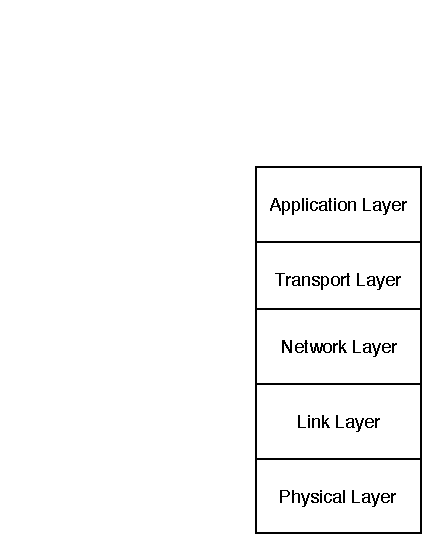
\includegraphics[scale = 1.2]{IPStack}
	\caption{IP Stack Layers}
	\label {ipstack}
\end{figure}


FTP is built on TCP/IP, and is therefore a reliable connection protocol. This project uses socket programming in order to implement FTP. Sockets can be viewed as the \textit{door} connecting the application and transport layers, as seen in Fig~\ref{socket}. The socket programs which are used to make the protocol use TCP and IP (which is beyond the scope of this project). 

FTP uses a set of commands and protocols in order order to achieve desired outcome, for example, a client has to send a password along with a specific command to the server in order for the input password to be valid. Upon receiving a said command, the server replies with a code number, accompanied by text, that indicates the failure or success of the implementation of said command. 


For this project, multi-threading was used. Muti-threading allows for the same code to run in different instances, effectively allowing the same code to run independently in different processes of the computer. For this project, multi-threading is used on the server side in order to allow different clients that connect to the server to run independently on different processes of the server. The detailing of threading falls out of the scope of this project, there is however literature that discuss threading such as reference~\cite{fop}.


As mentioned above, FTP is built on TCP/IP. TCP is a transport layer protocol whose fundamental task is the transmission of data between hosts~\cite{cn,mg}.

\begin{figure}[hbtp!]
	\centering
	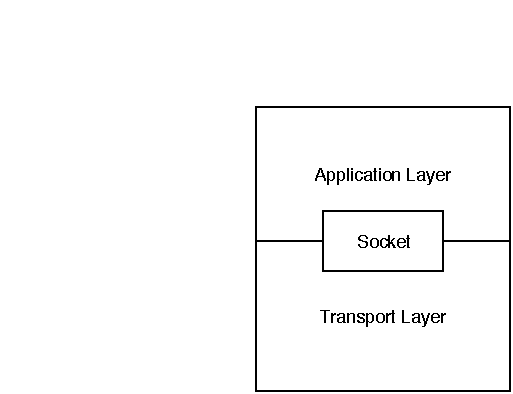
\includegraphics[scale = 1.2]{socket}
	\caption{IP Stack Layers}
	\label {socket}
\end{figure}


Wireshark was also used to monitor the packets when operating FTP.

In order to store passwords and user names, a database needs to be used on the server side. The author opted to use MySQL database because of its security and reliability. The database has a single table which is used to store the user name, user password, and the root directory for the said user wherein the user can perform file transfers on the server side. Due to MySQL using SQL, queries can be easily performed. An example of a useful query would be to find out if the user name, which is used in logging in when using FTP, exists~(see Fig~\ref{qu}). If the user name exists, then the server proceeds to request for the user password,etc.

\begin{figure}[hbtp]
	%\raggedleft
	\begin{lstlisting}
	select count(*) from user 
	where name = some_password
	\end{lstlisting}
	\caption{Querying whether user name exists}
	\label {qu}
\end{figure}



\subsection{Project Requirements}
The project requirements of the FTP program is the following:

\begin{itemize}
	\item  Implementation of FTP client code basic features
	\item  Implementation of FTP server code basic features
	\item  Using multi-threading
	\item  Ability to deal with different types of files
	\item  Use different computers for file transferring
	\item  Using wireshark
\end{itemize}

\section{Design and Implementation}
The design and implementation of the authors' FTP program is in three parts. The parts are the client code, server code and MySQL database table. This section discusses the three mentioned parts and their implementation.

\subsection{Database}

Databases are useful for storing information. The authors opted to use MySQL database because of the simplicity of use and the author's experience with it. A table called \textbf{user} is created in the database~(that is, MySQL) using the syntax shown in Fig~\ref{sqltable}. The table stores the user name, password of the user and the root name. The root name serves as a root directory for a user. Each root name therefore necessarily has to be unique for each user. By having unique root directory names, it is ensured that multiple users can access and use the FTP server, via the FTP client program, without affecting the data of other users. This results in ensuring that the FTP program can service multiple users as well. Due to the fact that the aforementioned table is created in using SQL~(MySQL is a SQL database), all queries performed use SQL.

\begin{figure}[hbtp]
	%\raggedleft
	\begin{lstlisting}
	create table user(
	user_name char(50),
	password char (50),
	root char (50),
	primary key(50)
	);
	\end{lstlisting}
	\caption{SQL code for creating a table for storing credentials}
	\label {sqltable}
\end{figure}

A visual example of this table is shown in Table~\ref{tasks}. The SQL queries that are performed in the authors' FTP  program are performed on this table. Storing the user credentials in a database instead of another storage format was chosen because of the following reasons. Firstly, by storing the data in a database ensures that the data is safely stored regardless of whether the server code is active or not. The use of the database also allows one to easily query data. Based on the authors' experience it was concluded that querying text files, csv files, etc results in very complex code. Due to the database already using a language~(that is, SQL), the amount of code necessary to perform a query is significantly reduced. Integrating the database with python is also simple. One of the major factors for using a database is that the data can be accessed across the entire server program, whether in functions, modules and/or classes. The benefit of such accessibility is if/when working with multiple python script files, the data can be accessed without having to make provision for passing data between the scripts that may need it. This in turn, results in the server code being easily scalable in terms of having multiple users.






\begin{figure}[hbtp]
	%\raggedleft
	\begin{lstlisting}
	select count (*) 
	where user_name = someUserName
	\end{lstlisting}
	\caption{SQL code for checking if user exists}
	\label {sqluser}
\end{figure}

When the user enters the credentials stored in the database,  queries have to be performed on the database, in order to ensure that the correct user is logging in, and to dictate which root directory~(which is based on the root name column of Table~\ref{tasks}) a user can use when operating the FTP program. The basic queries that need to be performed on the table~(or database) are ones for user name verification, password verification and root name access.

\begin{figure}[hbtp]
	%\raggedleft
	\begin{lstlisting}
	select count (*) 
	where user_name = someUserName
	and password = somePassword
	\end{lstlisting}
	\caption{SQL code for checking if the password matches the user name}
	\label {sqlpass}
\end{figure}

When a user enters their \textit{unique} user name, a query that determines whether the user name exists in the database is executed. The SQL code example for this query is given in Fig~\ref{sqluser}. Due to the fact that each user name will be unique, when the query runs it returns either a one or a zero. When the result is a one, it means that the same user name exists in this query. When the result is zero, it means that the user name does not exist, that is, the login account does not exist.

\begin{figure}[hbtp]
	%\raggedleft
	\begin{lstlisting}
	select root from user
	where user_name = someUserName
	\end{lstlisting}
	\caption{SQL code for assigning root directory name for said user}
	\label {sqlroot}
\end{figure}

Fig~\ref{sqlroot} is SQL code that returns a root folder name  for a specified user, the returned user name is used to determine the root directory of said user, as stated above. Fig~\ref{sqlpass} shows the generic SQL code that returns the number of user names where the password entered on the client side matches the one stored in the databases' user table. Due to the fact that the user names of the table always unique, if the number returned by the query is the number one, then it means the password for said user name is correct. If the returned value is zero, then it means that the password is incorrect. It is important to note that the code given in Fig~\ref{sqlpass} is only ever run if the entered user name queried in Fig~\ref{sqluser} exists. Due to this, the entered user name is always correct, and only the password authenticity is tested.



\begin{table}[hbtp!]
	\caption{Table design of SQL Database for user credentials}
	\label{tasks}
	\begin{center}
		\begin{tabular}{| c | c | c |}
			%\multicolumn{2}{|c|}{Software and Hardware Tools}\\
			\hline
			user-name & password & root\\
			\hline
			user1 & pass1 & root1\\
			\hline
			user2 & pass2 & root2\\
			\hline
			user3 & pass3 & root3\\
			\hline
			user4 & pass4 & root4\\
			\hline
		\end{tabular}
	\end{center}
\end{table}

\subsection{Server}
The server uses the database and queries it for user credentials and for determining root folders of each individual user, as stated above. The use of the database is embedded in the server's functions, modules, etc. This section focuses on an abstracted level of how the server interacts with the client code as demonstrated in Algorithm~\ref{serveralg1}. 

This section abstractly explains how the server is designed, and uses Algorithm~\ref{serveralg1}'s pseudocode to explain it. Based on Algorithm~\ref{serveralg1}'s pseudocode, it is seen that the server first connects to the database in order to enable it to make queries to the database. Once database connections are established, the server then waits for client programs to make connections to it. Once a client programs connects to the server, a thread for servicing said client program is established. From this point on, how the server operates is essentially by taking in input commands from the client and processing them, and then performing the necessary task based on the command received and then sending replies back to the client. This design pattern is followed by the server whether it be when logging in, entering passwords or downloading a file.


	\begin{algorithm}
	\caption{Server Algorithm}\label{serveralg1}
	\begin{algorithmic}[1]
		\Procedure{Processing Client Commands}{}
		
		connectDatabase()
		
		startSocketConnection()
		
		\While{True:} {
		\EndWhile
		
	
		createThread()
		
		command $\gets$ receiveCommand()
		
		commandType $\gets$ extractCommandType (command)
		
		commandValue $\gets$ extractCommandValue (command)
		
		\If{loggedIn() == false} 
			getCorrectLoginDetails (commandType, commandValue)
		\Else~processCommand(commandType, commandValue)
		\EndIf
		
		}
		 
		\EndProcedure
	\end{algorithmic}
\end{algorithm}

%%%%%%%%%%%%%%%%%%%%%%%%%%%%%



%%%%%%%%%%%%%%%%%%%%%%%%%%%%%%


\subsection{Client}
Algorithm~\ref{clientalg1} shows the high level pseudocode of how clients interact with the server. The client program first makes a connection to the server. Then after that the user enters commands to the client. The client then sends the commands to the client and the server responds to the client based  on the input it receives. The client then proceeds to process these commands. 
\begin{algorithm}
	\caption{Client Algorithm}\label{clientalg1}
	\begin{algorithmic}[1]
		\Procedure{Processing Server Commands}{}
		
		connectToServer()
		\While {command != 'QUIT':}{
		
		
		command $\gets$ getUserInputCommand()
		
		sendCommandToServer(command)
		
		response $\gets$ getServerResponse()
		
		responseCode $\gets$ extractResponseCode(response)
		
		processResponse (response, responseCode)
		
		\EndWhile
		}
		\EndProcedure
	\end{algorithmic}
\end{algorithm}


\subsection{Commands and Reply Codes}


\section{Code Functionality}



\section{Testing and Results}


% Include wireshark screenshots

\section{SWAT Analysis}

This section provides a SWAT analysis to the FTP program based on what the authors implemented. 

\subsection{Strengths}
Most of the basic FTP commands were successfully implemented. The program is also easily scalable due to its design.

\subsection{Weaknesses}
Some of the basic features of the program for FTP were not implemented. The program does not make use of a GUI and therefore, cannot interact with FileZilla. 

\subsection{Advantages}
The code is simple to use and the program provides detailed error codes to inform the user what their error is.


\subsection{Trade-offs}
Some of the basic commands of FTP were not implemented because they were seen as redundant, as such, the authors chose to implement less commands and limited functionality in order to have a running code that has less chances of an error. 


\section{Division of Tasks}

Due to the project requiring that a division of tasks be given, the authors opted code one python script each. Uyanda Mphunga implemented the server script and Ashraf Omar implemented the client side.

\section{Future Improvements}

For future improvements, a GUI needs to be implemented, and perhaps also allow for the neglected commands to be implemented.

\section{Conclusion}

%%%%%%%%%%%%%%%%%%%%%%%%%%%%%%%%%%%%%%%%%%%%%%%%%%%%%%%%%%%%%%%%%%%%%%%%%%%%%%%
%
%\nocite{*}
\onecolumn
\bibliographystyle{IEEEtran}
\bibliography{networks}

%{\tiny \vfill \hfill \today \hspace{5mm} witseie-paper-2003.\TeX}

\end{document}